\documentclass{article} % For LaTeX2e
\usepackage{iclr2018_conference,times}
\usepackage{hyperref}
\usepackage{url}

\usepackage{booktabs}       % professional-quality tables
\usepackage{nicefrac}       % compact symbols for 1/2, etc.
\usepackage{microtype}      % microtypography

\usepackage{wrapfig}
\usepackage{graphicx} % more modern
\usepackage{caption}
\usepackage{subcaption}

\usepackage{algorithm}
\usepackage{algorithmic}



% AMS stuff
\usepackage{amsmath, amssymb}
\usepackage{dsfont}

%\usepackage{ntheorem}
\usepackage[amsthm,thmmarks]{ntheorem}

\newtheorem{theorem}{Theorem}
\newtheorem{lemma}{Lemma}
\newtheorem{cor}{Corollary}
\newtheorem{proposition}{Proposition}

\DeclareMathOperator*{\argmin}{arg\,min}
\DeclareMathOperator*{\argmax}{arg\,max}
\usepackage{xspace}
\newcommand*{\eg}{e.g.\@\xspace}
\newcommand*{\ie}{i.e.\@\xspace}

%\usepackage[usenames, dvipsnames]{color}
\definecolor{myblue}{RGB}{1, 130, 180}
\definecolor{myred}{RGB}{214, 60, 55}


\title{Active Learning for Convolutional Neural Networks: A Core-Set Approach}

% Authors must not appear in the submitted version. They should be hidden
% as long as the \iclrfinalcopy macro remains commented out below.
% Non-anonymous submissions will be rejected without review.

\author{Antiquus S.~Hippocampus, Natalia Cerebro \& Amelie P. Amygdale \thanks{ Use footnote for providing further information
about author (webpage, alternative address)---\emph{not} for acknowledging
funding agencies.  Funding acknowledgements go at the end of the paper.} \\
Department of Computer Science\\
Cranberry-Lemon University\\
Pittsburgh, PA 15213, USA \\
\texttt{\{hippo,brain,jen\}@cs.cranberry-lemon.edu} \\
\And
Ji Q. Ren \& Yevgeny LeNet \\
Department of Computational Neuroscience \\
University of the Witwatersrand \\
Joburg, South Africa \\
\texttt{\{robot,net\}@wits.ac.za} \\
\AND
Coauthor \\
Affiliation \\
Address \\
\texttt{email}
}

% The \author macro works with any number of authors. There are two commands
% used to separate the names and addresses of multiple authors: \And and \AND.
%
% Using \And between authors leaves it to \LaTeX{} to determine where to break
% the lines. Using \AND forces a linebreak at that point. So, if \LaTeX{}
% puts 3 of 4 authors names on the first line, and the last on the second
% line, try using \AND instead of \And before the third author name.

\newcommand{\fix}{\marginpar{FIX}}
\newcommand{\new}{\marginpar{NEW}}

%\iclrfinalcopy % Uncomment for camera-ready version, but NOT for submission.

\begin{document}


\maketitle

\begin{abstract} 
Convolutional neural networks (CNNs) have been successfully applied to many recognition and learning tasks using a universal recipe;
    training a deep model on a very large dataset of supervised examples. However, this approach is rather restrictive in practice since collecting a
    large set of labeled images is very expensive. One way to ease this problem is coming up with smart ways for choosing images to be labelled from a
    very large collection (\ie active learning).

    Our empirical study suggests that many of the active learning heuristics in the literature are not effective when applied to CNNs. Inspired by these results, we define the problem of active learning as \emph{core-set selection}, \ie choosing set of points such that a model learned over the selected subset is competitive for the remaining data points. We further present a theoretical result characterizing the performance of any selected subset using the geometry of the datapoints. As an active learning algorithm, we choose the subset which is expected to yield best result according to our characterization. Our experiments show that the proposed method significantly outperforms existing approaches in image classification experiments by a large margin. 
\end{abstract} 

\section{introduction}
Deep convolutional neural networks (CNNs) have shown unprecedented success in many areas of research in computer vision and pattern recognition, like
image classification, object detection, and scene segmentation. Although CNNs are universally successful in many tasks, they have a major drawback;
they need a very large amount of labeled data to be able to learn their millions of parameters. More importantly, it is almost always better to have
more data since the accuracy of CNNs is often not saturated with increasing dataset size. Hence, there is a constant desire to collect more and more
data. Although this is the behavior you want from an algorithmic perspective (higher representative power is typically better), labeling a dataset is
a time consuming and an expensive task. These practical considerations raise a critical question: \emph{``what is the optimal way to choose data
points to label such that the highest accuracy can be obtained given a fixed labeling budget.''} Active learning is one of the common paradigms to
address this question.

The goal of active learning is to find effective ways to choose data points to label, from a pool of unlabeled data points, in order to maximize the
accuracy. Although it is not possible to obtain a universally good active learning strategy \citep{dasgupta2004analysis}, there exist many
heuristics~\citep{settles2010active} which have been proven to be effective in practice. Active learning is typically an iterative process in which a
model is learned at each iteration and a set of points is chosen to be labelled from a pool of unlabelled points using these aforementioned heuristics. We experiment
with many of these heuristics in this paper and find them not effective when applied to CNNs. We argue that
the main factor behind this ineffectiveness is the correlation caused via batch acquisition/sampling. In classical setting, the active learning algorithms
typically choose a single point at each iteration; however, this is not feasible for CNNs since i) a single point is likely to have no statistically
significant impact on the accuracy due to the local optimization methods, and ii) each iteration requires a full training until convergence which
makes it intractable to query labels one-by-one. Hence, it is necessary to query labels for a large subset at each iteration and it results in correlated samples even for
moderately small subset sizes.

In order to tailor an active learning method for the batch sampling case, we decided to define the active learning as \emph{core-set selection} problem. Core-set selection problem aims to find a small subset given a large labeled dataset such that a model learned over the small subset is competitive over the whole dataset. Since
we have no labels available, we perform the core-set selection without using
the labels. In order to attack the unlabeled core-set problem for CNNs, we provide a rigorous bound between an average loss over any subset of the dataset and
the remainder via the geometry of the data points. As an active learning algorithm, we try to choose a subset such that this bound is minimized. Moreover, minimization of this bound turns out to be equivalent to the k-Center problem~\citep{facility} and we adopt an efficient approximate solution to this 
combinatorial optimization problem. We further study the behavior of our proposed algorithm empirically for the problem of image classification using three different datasets. Our empirical analysis demonstrates state-of-the-art performance by a large margin. 


\section{Related Work} We discuss the related work in the following categories
separately. Briefly, our work is different from existing approaches since $i)$
it defines the active learning problem as core-set selection, $ii)$ we consider
both fully supervised and weakly supervised cases, and $ iii)$ we rigorously
address the core-set selection problem directly for CNNs with no extra
assumption. 


\noindent\textbf{Active Learning} Active learning has been widely studied and
most of the early work can be found in the classical survey
\citep{settles2010active}. It discusses most acquisition functions such as
information theoretical methods \citep{mackay1992information}, ensemble
approaches \citep{mccallumzy1998employing, freund1997selective} and uncertainty
based methods
\citep{tong2001support,lewissequential,joshi2009multi,li2013adaptive}.

Bayesian active learning methods typically use a non-parametric model like
Gaussian process to estimate the expected improvement by each query
\citep{kapoor2007active} or expected error after a set of queries
\citep{roy2001toward}. These approaches are not directly applicable to deep learning
scenarios since they do not scale to large-scale datasets. A recent approach by~\citet{gal_bayes} shows and equivalence between dropout and approximate
Bayesian inference enabling the application of Bayesian methods to deep
learning. Although Bayesian active learning has been shown to be effective
for small datasets \citep{gal_active}, our empirical analysis suggests that they do not scale to large-scale datasets because of batch sampling.

One important class is that of uncertainty based methods, which try to find hard
examples using heuristics like highest entropy \citep{joshi2009multi}, and
geometric distance to decision boundaries
\citep{tong2001support,brinker2003incorporating}. Our empirical analysis suggest them to be not effective for CNNs.


There are recent optimization based approaches which can trade-off uncertainty
and diversity to obtain a diverse set of hard examples. Elhamifar~et al.
\citep{elhamifar2013convex} design a discrete optimization problem for this
purpose and use its convex surrogate. However, the algorithm uses $n^2$
variables where $n$ is the number of data points. Hence, it does not scale to
the deep learning case. There are also many discrete optimization based active
learning algorithms designed for the specific class of machine learning
algorithms like k-nearest neighbors and naive Bayes \citep{wei2015submodularity}.
Even in the algorithm agnostic case, one can design a set-cover algorithm to
cover the hypothesis space using sub-modularity \citep{guillory2010interactive,
golovin2011adaptive}. Our algorithm can be considered to be in this class;
however, we do not use any uncertainty information. Our algorithm is also the
first one which applies to the CNNs. Most similar to ours is \citep{porikli},
using a similar optimization problem. However, they have no theoretical
justification or analysis. Moreover, it is also not experimented for the CNNs.

Recently, a discrete optimization based method \citep{BerlindU15} which is
similar to ours has been presented for k-NN type algorithms in the domain shift
setting. Although our theoretical analysis borrows some techniques from
\citep{BerlindU15}, their results are only valid for k-NN and are not applicable
to CNNs.

Recently, active learning algorithms for CNNs are presented in
\citep{wang2016cost, captcha}. \citet{wang2016cost} propose an heuristic based algorithm which directly assigns
labels to the data points with high confidence and queries labels for the ones
with low confidence. Moreover, \citet{captcha} specifically targets recognizing CAPTCHA images. Although their results are promising for CAPTCHA recognition, their acquisition strategy is not effective for general image classification problem. We discuss limitations of both approaches in Section~\ref{sec:exp}.

\noindent\textbf{Core-Set Selection} The closest literature to our
work is the problem of core-set selection since we define active learning as a
core-set selection problem. This problem considers a
fully labeled dataset and tries to choose a subset of it such that the model
trained on the selected subset will perform as closely as possible to the model
trained on the entire dataset. For specific learning algorithms, there are
methods like core-sets for SVM \citep{tsang2005core} and core-sets for k-Means
and k-Medians \citep{har2005smaller}. However, we are not aware of such method for CNNs.

The most similar algorithm to ours is the unsupervised subset selection
algorithm described in \citep{wei2013using}. It uses a facility location problem
to find a diverse cover for the dataset. Our algorithm differs in that it uses a
slightly different formulation of facility location problem. Instead of the
min-sum, we use the minimax \citep{facility} form of the facility location. More
importantly, we apply this algorithm for the first time to the problem of active
learning and provide theoretical guarantees for the CNNs.
 
\noindent\textbf{Weakly-Supervised Deep Learning} Our paper is also related to
semi-supervised deep learning since we experiment the active learning both in
the fully-supervised and weakly-supervised scheme. One of the early
weakly-supervised convolutional neural network algorithms was Ladder networks
\citep{ladder}. Recently, we have seen adversarial methods which can learn a data
distribution as a result of a two-player non-cooperative game
\citep{salimans2016improved,gan_original,dcgan}. These methods are further
extended to feature learning \citep{ali, bigan}. We use Ladder networks in our
experiments since adversarial architectures are notoriously hard to train. Our
algorithm is agnostic to the weakly-supervised learning algorithm choice and can
easily use any weakly-supervised or fully-supervised model.

\section{Problem Definition} In this section, we formally define the problem of active learning in batch setting and set
up the notation for the rest of the paper. We are interested in a $C$ class classification problem defined over a
compact space $\mathcal{X}$ and a label space  $\mathcal{Y}=\{1,\ldots,C\}$. We also consider a loss function
$l(\cdot,\cdot;\mathbf{w}):\mathcal{X}\times \mathcal{Y} \rightarrow \mathcal{R}$ parametrized over the hypothesis class
($\mathbf{w}$), e.g.\ parameters of the deep learning algorithm. We further assume class-specific regression functions
$\eta_c(\mathbf{x})=p(y=c|\mathbf{x})$ to be \mbox{$\lambda^\eta$-Lipschitz} continuous for all $c$.

We consider a large collection of data points which are sampled $i.i.d.$ over the space
$\mathcal{Z}=\mathcal{X}\times\mathcal{Y}$ as \mbox{$\{\mathbf{x}_i,y_i\}_{i \in [n]} \sim p_\mathcal{Z}$} where
$[n]=\{1,\ldots,n\}$. We further consider an initial pool of data-points chosen uniformly at random as
\mbox{$\mathbf{s}^0=\{s^0(j) \in [n]\}_{j \in [m]}$}.

An active learning algorithm only has access to $\{\mathbf{x}_i\}_{i \in [n]}$ and $\{y_{s(j)}\}_{j \in [m] }$. In other
words, it can only see the labels of the points in the initial sub-sampled pool. It is also given a budget $b$ of
queries to ask an oracle, and a learning algorithm $A_{\mathbf{s}}$ which outputs a set of parameters $\mathbf{w}$ given
a labelled set $\mathbf{s}$. The active learning with a pool problem can simply be defined as 

\begin{equation} \min_{\mathbf{s}^1 : |\mathbf{s}^1| \leq b} E_{\mathbf{x},y \sim p_\mathcal{Z}} [l(\mathbf{x},y;
A_{\mathbf{s}^0 \cup \mathbf{s}^1})] \end{equation} 

In other words, an active learning algorithm can choose $b$ extra points and get them labelled by an oracle to minimize
the future expected loss. There are a few differences between our formulation and the classical definition of active
learning. Classical methods consider the case in which the budget is 1 ($b=1$) but a single point has negligible effect
in a deep learning regime hence we consider the batch case. It is also very common to consider multiple rounds of this
game. %as in each round $k$,% solving the following
%\begin{equation} \min_{\mathbf{s}^{k+1} : |\mathbf{s}^{k+1}| \leq b} E_{\mathbf{x},y \sim p_\mathcal{Z}}
%[l(\mathbf{x},y;A_{\mathbf{s}^{0} \cup \ldots  \mathbf{s}^{k+1} \cup \ldots  \mathbf{s}%^{k+hor}})] \end{equation}
%Where $hor$ is the number of active learning iterations expected to be performed. Although it is more realistic,
%analysis is typically trickier in such a setting. Hence, 
We also follow the multiple round formulation with a myopic approach by solving the single round of labelling as;
\begin{equation} \min_{\mathbf{s}^{k+1} : |\mathbf{s}^{k+1}| \leq b} E_{\mathbf{x},y \sim p_\mathcal{Z}}
[l(\mathbf{x},y;A_{\mathbf{s}^{0} \cup \ldots  \mathbf{s}^{k+1}})] \end{equation}
%Our method solves the multi-stage problem in a myopic way without utilizing look-ahead. 
We only discuss the first iteration where $k=0$ for brevity although we apply it over multiple rounds. 

At each iteration, an active learning algorithm has two stages: 1. identifying a set of data-points and presenting them
to an oracle to be labelled, and 2. training a classifier using both the new and the previously labeled data-points. The
second stage (training the classifier) can be done in a fully or weakly-supervised manner. Fully-supervised is the case
where training the classifier is done using only the labeled data-points. Weakly-supervised is the case where training
also utilizes the points which are not labelled yet. Although the existing literature only focuses on the active
learning for fully-supervised models, we considered both cases and experimented on both. 

\section{Method}
\subsection{Active Learning as a Set Cover} When there is no direct measure of uncertainty over the hypothesis class, the
active learning problem is typically considered as refining decision boundaries by querying hard examples. Hence, using
uncertainty is an empirically proven heuristic. However, this heuristic is typically effective when data points are fed
one by one (\ie $b=1$). Unfortunately, this is not feasible while training CNNs since $i)$ a single point will not have
a statistically significant impact on the model since the optimization algorithm is local. $ii)$ it is infeasible to
train as many models as number of points since many practical problem of interest is very large-scale.

Instead, we propose to define active learning problem as a core-set selection problem. Consider the following upper
bound of the optimization problem of interest;

\begin{equation} \begin{aligned} E_{\mathbf{x},y \sim p_\mathcal{Z}} [l(\mathbf{x},y; A_{\mathbf{s}^0 \cup
    \mathbf{s}^1})]  &\leq \underbrace{\left| E_{\mathbf{x},y \sim p_\mathcal{Z}} [l(\mathbf{x},y; A_{\mathbf{s}^0 \cup
    \mathbf{s}^1})] - \frac{1}{n}\sum_{i \in [n]} l(\mathbf{x}_i,y_i,A_{\mathbf{s}^0 \cup \mathbf{s}^1}) \right|}_{\text{Generalization Error}} \\ &+
    \underbrace{\left| \frac{1}{n}\sum_{i \in [n]} l(\mathbf{x}_i,y_i,A_{\mathbf{s}^0 \cup \mathbf{s}^1}) -
    \frac{1}{|\mathbf{s}^0+\mathbf{s}^1|}\sum_{j \in \mathbf{s}^0 \cup \mathbf{s}^1} l(\mathbf{x}_j,y_j;A_{\mathbf{s}^0 \cup \mathbf{s}^1}),
    \right|}_{\text{Core-Set Loss}} \\ &+ \underbrace{\frac{1}{|\mathbf{s}^0+\mathbf{s}^1|}\sum_{j \in
\mathbf{s}^0 \cup \mathbf{s}^1} l(\mathbf{x}_j,y_j,A_{\mathbf{s}^0 \cup \mathbf{s}^1})}_{\text{Training Error}} \end{aligned} \end{equation} 

Basically, the quantity we are interested in is related to generalization error, the loss of the core-set and the
training error. We already now empirically that CNNs are highly expressive leading to very low training error and they
typically generalize well for various visual problem. Hence. we are directly interested in the core-set loss for the
active learning problem. Hence, we re-define the active learning as the following optimization problem:


\begin{equation} \min_{\mathbf{s}^1 : |\mathbf{s}^1| \leq b} 
\left| \frac{1}{n}\sum_{i \in [n]} l(\mathbf{x}_i,y_i,A_{\mathbf{s}^0 \cup \mathbf{s}^1}) -
    \frac{1}{|\mathbf{s}^0+\mathbf{s}^1|}\sum_{j \in \mathbf{s}^0 \cup \mathbf{s}^1} l(\mathbf{x}_j,y_j;A_{\mathbf{s}^0 \cup \mathbf{s}^1}),
    \right|
    \label{eq:new_active_learning}
\end{equation} 

\subsection{Core-Sets for CNNs}
In this section, we explain how we solve the core-set problem for CNNs. Specifically, we are interested in solving the
optimization problem defined in (\ref{eq:new_active_learning}). This optimization function is not tractable since we
only have an access of the labels of the initial pool $\mathbf{s}^0$. In other words, $y_i, i \in [n] \setminus
\mathbf{s}^0$ is not visible to us and we can only query the labels for budget number of data points as $\mathbf{s}^1$.

In order to solve this problem, we use the regularities of the loss functions of the CNNs. We start with providing an
upper bound for (\ref{eq:new_active_learning}) for the case of CNNs with no unrealistic assumption. We start with
first finding this bound for any Lipschitz loss function and then show that loss functions of CNNs are Lipschitz when
only the ReLu non-linearity is used. We provide the following proposition for any Lipschitz loss function and visualize
it in Figure~\ref{fig:thm}.

\begin{theorem} Given $n$ i.i.d. samples drawn from $p_\mathcal{Z}$ as $\{\mathbf{x}_i,y_i\}_{i\in[n]}$, and set of
    points $\mathbf{s}$. If loss function $l(\cdot,y,\mathbf{w})$ is $\lambda^l$-Lipschitz continuous
    for all $y, \mathbf{w}$ and bounded by $L$, regression function is $\lambda^\eta$-Lipschitz, $\mathbf{s}$
    is $\delta_\mathbf{s}$ cover of $\{\mathbf{x}_i,y_i\}_{i\in[n]}$, and
    $l(\mathbf{x}_{s(j)},y_{s(j)},A_\mathbf{S})=0\quad \forall j \in [m]$; with probability at least $1-\gamma$,
    \begin{small} \[
%\frac{1}{n}\sum_i l(\mathbf{x}_i,y_i,A_\mathbf{s}) \leq \mathcal{L}_{[n]} (h^\star) +\delta(\lambda^l + 2
            %\lambda^{\eta}) + \sqrt{\frac{\log(1/1-\gamma)}{2n}}
\frac{1}{n}\sum_{i \in [n]} l(\mathbf{x}_i,y_i) \leq \delta (\lambda^l + \lambda^\mu LC)+ \sqrt{\frac{L^2
    \log(1/\gamma)}{2n}}. \] \end{small}
%where $\mathcal{L}_{[n]} (h^\star)$ is the loss of the Bayes-optimal classifier.
\label{mainthm2} \end{theorem}

\begin{figure}[ht]
    \begin{center} 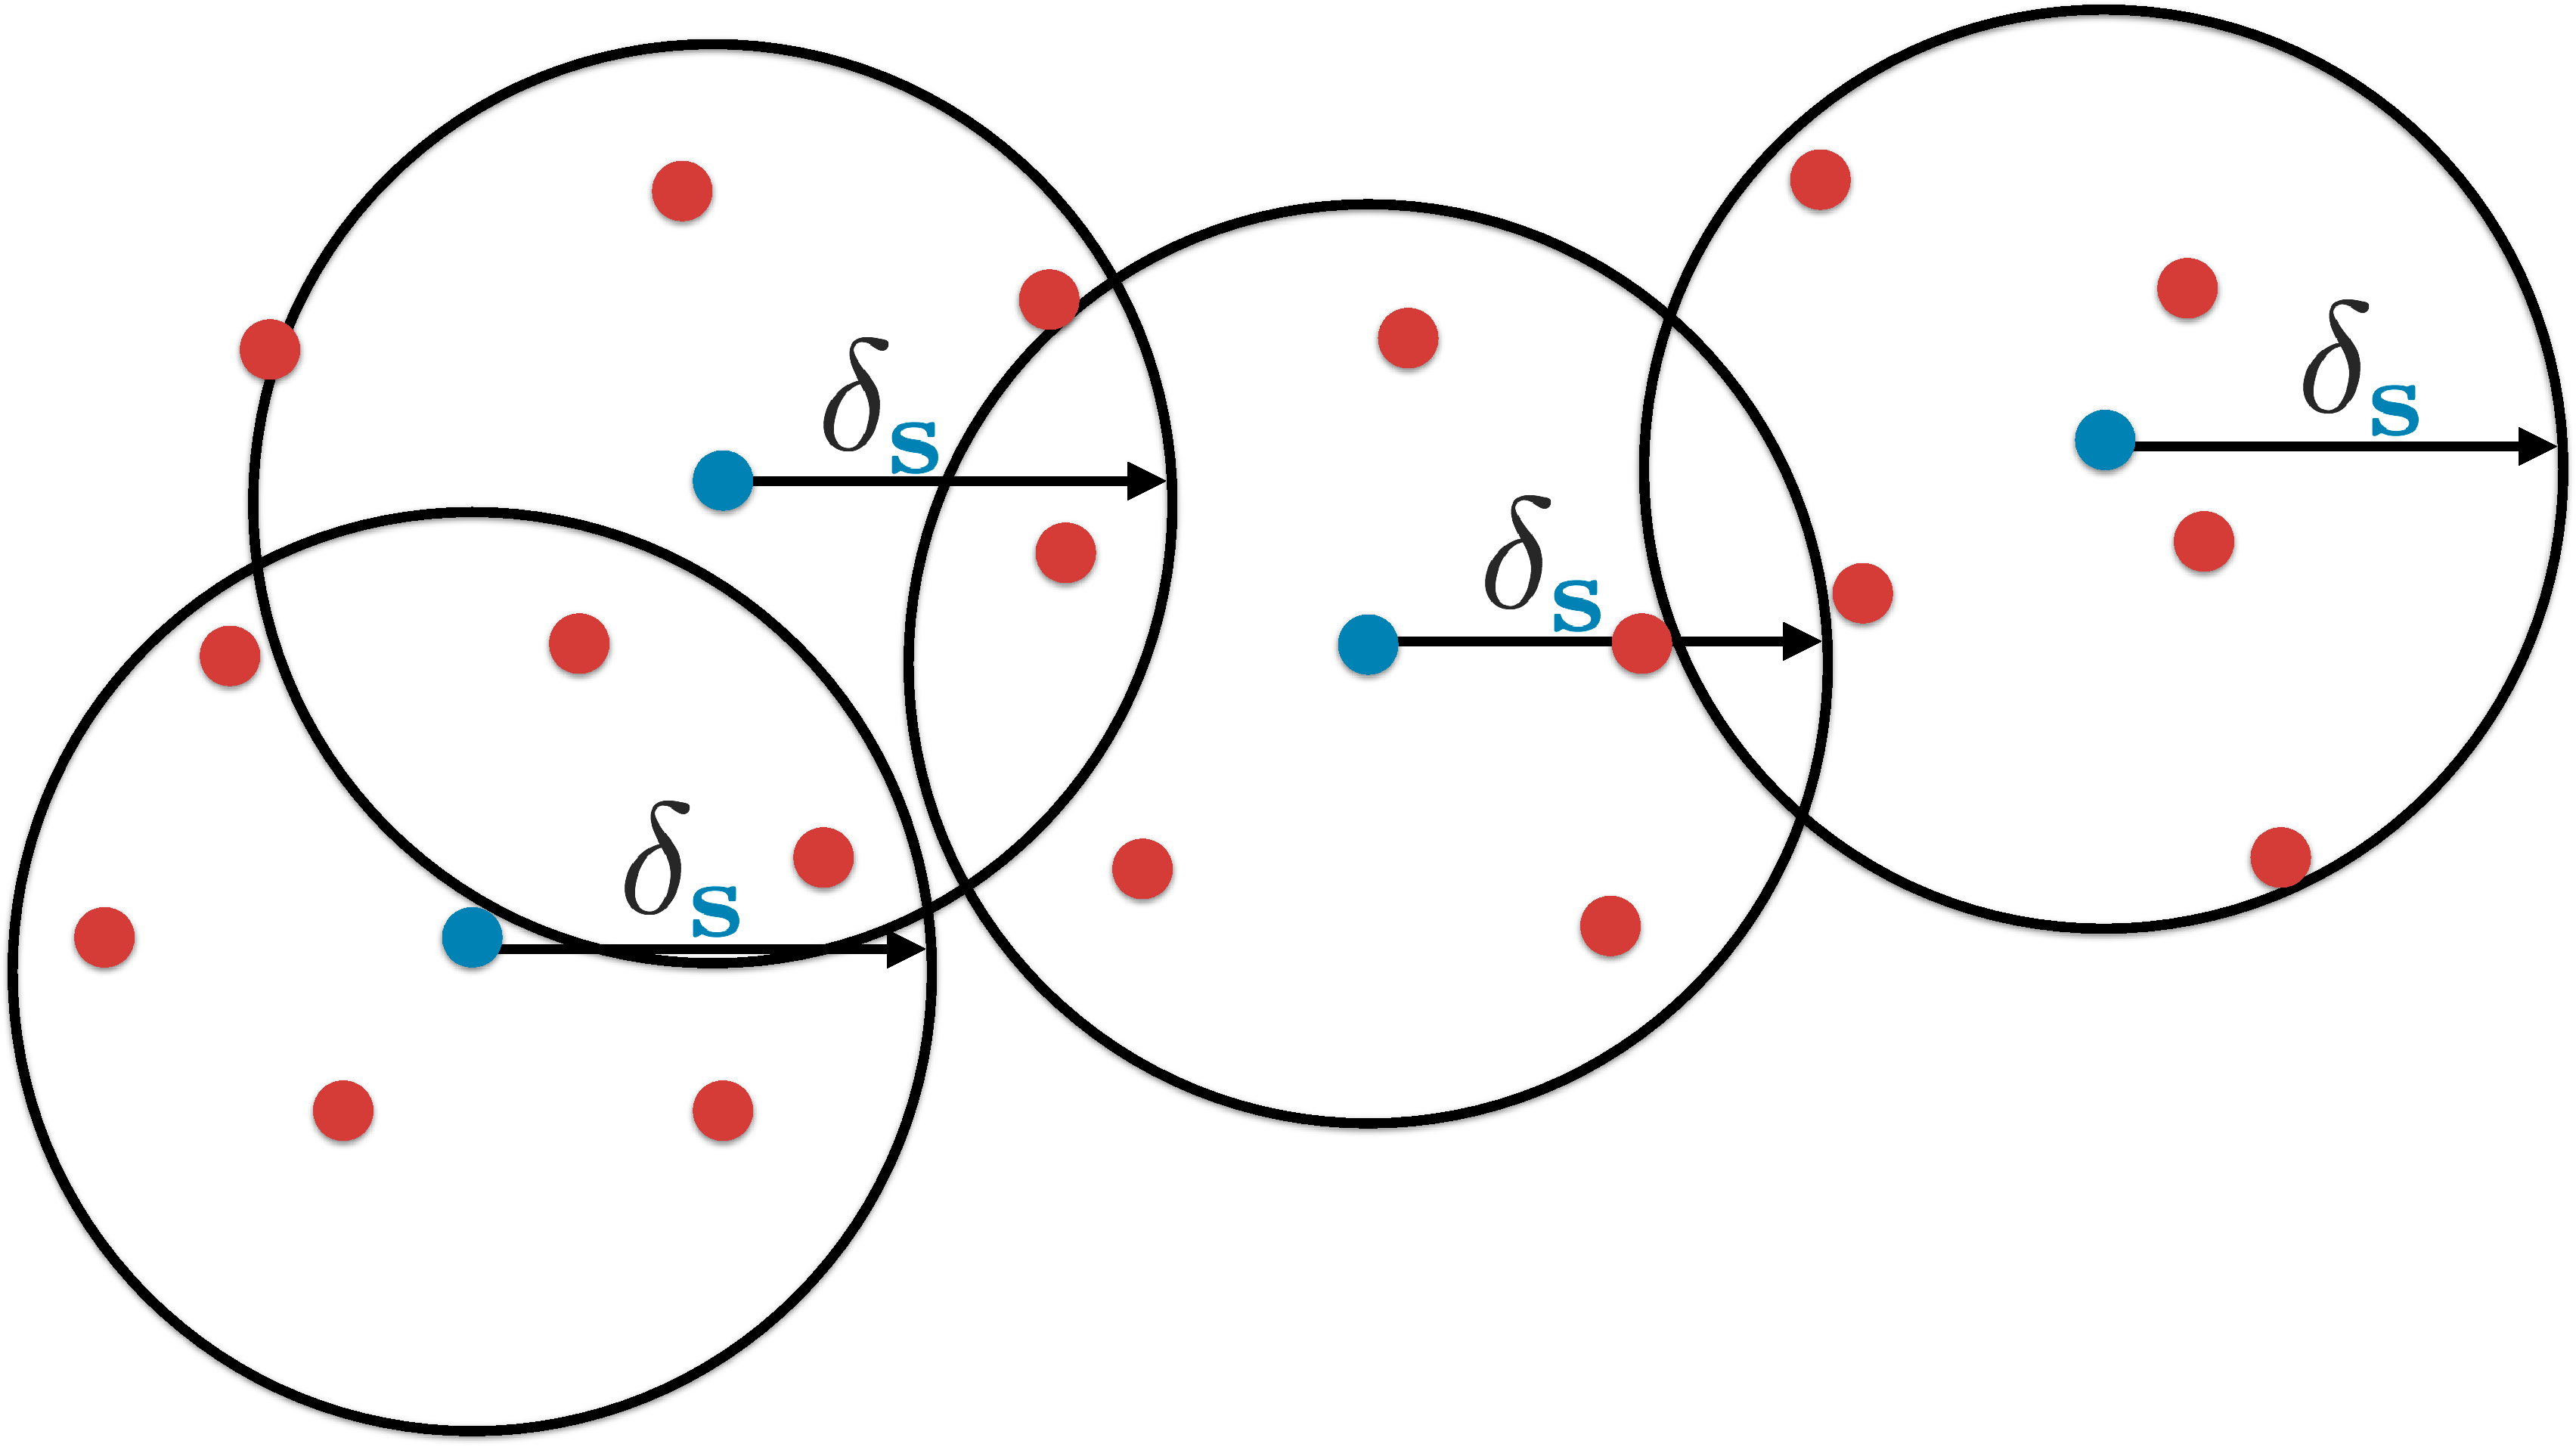
\includegraphics[width=0.8\textwidth]{thm.pdf} \end{center} 
        \caption{\textbf{Visualization of the Proposition \ref{mainthm2}}. Consider the set of selected points
        {\color{myblue} $\mathbf{s}$} and the points in the remainder of the dataset {\color{myred} $[n] \setminus
        \mathbf{s}$}, our results shows that if $\mathbf{s}$ is the $\delta_{\mathbf{s}}$ cover of the dataset, 
        $\left| {\color{myred} \frac{1}{n}\sum_{i \in [n]} l(\mathbf{x}_i,y_i,A_{\mathbf{s}})} -{\color{myblue} \frac{1}{|\mathbf{s}|}\sum_{j \in
        \mathbf{s}} l(\mathbf{x}_j,y_j;A_{\mathbf{s}})}
    \right| \leq \mathcal{O}\left(\delta_\mathbf{s}\right) + \mathcal{O}\left(\sqrt{\frac{1}{n}}\right)$}
    \label{fig:thm}
    \end{figure}

First of all, this proposition is applicable to any machine learning algorithm with a Lipschitz loss function and we
further prove the Lipschitz-continuity of CNNs. It can clearly be seen that the empirical loss converges to the expected
loss with large number of data points $n$ since $\lambda^l\epsilon$ term can be made arbitrarily small. In order to
complete the study about the generalization performance of CNNs, we prove the Lipschitz-continuity of the loss function
of a CNN with the following lemma where max-pool and restricted linear units are the non-linearities and the loss is
defined as the $l_2$ distance between the desired probabilities and the soft-max outputs.

\begin{lemma} A convolutional neural network with $n_c$ convolutional (with max-pool and ReLU) and $n_{fc}$ fully
connected layers defined over C classes with loss function defined as the 2-norm between the softmax output and class
probability is $\left(\frac{\sqrt{C-1}}{C} \alpha^{n_c+n_{fc}}\right)$-Lipschitz. \end{lemma}

Here, $\alpha$ is the maximum sum of  input weights per neuron (see appendix for formal definition). Although it is in
general unbounded, it can be made arbitrarily small without changing the loss function behavior (\ie keeping the label
of any data point $\mathbf{s}$ unchanged). % since dividing all weights with a scalar will not switch any label. Hence,
for any CNN, there is an equivalent CNN (in terms of classification function) with $\alpha \leq \varrho$ for any
$\varrho > 0$. We can conclude that CNNs enjoy a $0$ generalization error in the limiting case thanks to the Lipschitz
property.

In order to perform active learning, we simply use this upper bound of the optimization function we are interested in.
Hence, the practical problem of interest becomes $\min_{\mathbf{s}^1:|\mathbf{s}^1 \leq b|} \delta_{\mathbf{s}^0\cup
\mathbf{s}^1}$. This problem is equivalent to the k-Center problem which is also called as min-max facility location
problem \citep{k-center}. In the next section, we explain how do we solve the k-Center problem in practice usign greedy
approximation following the classical method in the literature.

\newpage

\subsection{Solving the k-Center Problem} 
\label{sec:alg} 
\begin{wrapfigure}{R}{0pt}
\begin{minipage}{0.44\textwidth}
\vspace{-8mm}
   \begin{algorithm}[H] 
   \caption{k-Center-Greedy} 
   \label{alg:greedy} 
   \begin{algorithmic} 
   \STATE {\bfseries Input:} data $\mathbf{x}_i$, existing pool $\mathbf{s}^0$ and a budget $b$ 
   \STATE Initialize $\mathbf{s}=\mathbf{s}^0$ \REPEAT \STATE $u=\arg\max_{i \in [n] \setminus \mathbf{s}} \min_{j \in \mathbf{s}} \Delta(\mathbf{x}_i, \mathbf{x}_j)$ \STATE $\mathbf{s} = \mathbf{s} \cup \{u\}$ 
   \UNTIL {$|\mathbf{s}|=b+|\mathbf{s}^0|$} 
   \STATE {\bfseries return} $\mathbf{s} \setminus \mathbf{s}^0$ \end{algorithmic}
\end{algorithm} 
\vspace{-10mm}
\end{minipage} 
\end{wrapfigure}
We provided an upper bound for the loss function of the core-set selection problem and showed that minizinig it is equivalent to the \emph{k-Center} problem (minimax facility location \citep{facility}) which can intuitively be defined as follows; choose $b$ center points such that the  largest distance between a data point and its nearest center is minimized. Formally, we are trying to solve: 
\begin{equation}
    \min_{\mathbf{s}^1:|\mathbf{s}^1| \leq b} \max_i \min_{j \in \mathbf{s}^1 \cup \mathbf{s}^0} \Delta(\mathbf{x}_i,\mathbf{x}_j)
\end{equation}

Unfortunately this problem is NP-Hard \citep{cook}. However, it is possible to obtain a $2-OPT$ solution efficiently
using a greedy approach shown in  Algorithm~\ref{alg:greedy}. If $OPT=\min_{\mathbf{s}^1} \max_i \min_{j \in
\mathbf{s}^1 \cup \mathbf{s}^0} \Delta(\mathbf{x}_i,\mathbf{x}_j)$, the greedy algorithm shown in
Algorithm~\ref{alg:greedy} is proven to have a solution ($\mathbf{s}^1$) such that; $ \max_i \min_{j \in \mathbf{s}^1
\cup \mathbf{s}^0} \Delta(\mathbf{x}_i,\mathbf{x}_j) \leq 2 \times OPT$.


Although the greedy algorithm gives a good initialization, in practice we can improve the $2-OPT$ solution by
iteratively querying upper bounds on the optimal value. In other words, we can design an algorithm which decides if $OPT
\leq \delta$. In order to do so, we define a mixed integer program (MIP) parametrized by $\delta$ such that its
feasibility indicates $\min_{\mathbf{s}^1} \max_i \min_{j \in \mathbf{s}^1 \cup \mathbf{s}^0}
\Delta(\mathbf{x}_i,\mathbf{x}_j) \leq \delta$. A straight-forward algorithm is using this MIP as a sub-routine and
performing a binary search between the result of the greedy algorithm and its half since the optimal solution is
guaranteed to be included in that range. While constructing this MIP, we also try to handle one of the weaknesses of
k-Center algorithm, namely robustness. To make the k-Center problem robust, we assume an upper limit on the number of
outliers $\Xi$ such that our algorithm can choose not to cover at most $\Xi$ unsupervised data points. This mixed
integer program can be written as:

\begin{equation}
\begin{aligned}
Feasible(b,\mathbf{s}^0,\delta, \Xi):  &\sum_j  u_j, = |\mathbf{s}^0|+ b,  \quad &&  \sum_{i,j} \xi_{i,j} \leq \Xi \\
&\sum_j \omega_{i,j} = 1\quad \forall  i, \quad && \omega_{i,j} \leq u_j \quad \forall  i,j \\
   & u_j =1 \quad \forall j\in \mathbf{s}^0, \quad && \omega_{i,j} = \xi_{i,j} \quad  \forall i,j \mid   \Delta(\mathbf{x}_i,\mathbf{x}_j)  > \delta .
\end{aligned}\label{eq:mip}
\end{equation}

In this formulation, $u_i$ is 1 if the $i^{th}$ data point is chosen as center, $\omega_{i,j}$ is $1$ if the $i^{th}$
point is covered by the $j^{th}$, point and $\xi_{i,j}$ is 1 if the $i^{th}$ point is an outlier and covered by the
$j^{th}$ point without the $\delta$ constraint, and $0$ otherwise. And, variables are binary as $u_i, \omega_{i,j},
\xi_{i,j} \in \{0,1\}$. We further visualize these variables in a diagram in Figure~\ref{mip}, and give the details of
the method in Algorithm~\ref{alg:bin}. 

\begin{figure*}[h]
    \begin{minipage}[t]{0.5\textwidth}
    \vspace{-3mm} 
    \begin{algorithm}[H]
        \caption{Robust k-Center} 
        \label{alg:bin} 
        \begin{algorithmic} 
        \STATE {\bfseries Input:} data $\mathbf{x}_i$,
            existing pool $\mathbf{s}^0$, budget $b$ and outlier bound $\Xi$ 
         \STATE {\bfseries Initialize} $\mathbf{s}_g
            =$ k-Center-Greedy($\mathbf{x}_i, \mathbf{s}^0, b$) 
            \STATE $\delta_{2-OPT} = \max_j \min_{i \in
            \mathbf{s}_g} \Delta(\mathbf{x}_i,\mathbf{x}_j)$ 
            \STATE $lb=\frac{\delta_{2-OPT}}{2}$, $ub=\delta_{2-OPT}$
            \REPEAT \IF {$Feasible(b, \mathbf{s}^0,\frac{lb+ub}{2},\Xi)$} 
            \STATE $ub=\max_{i,j \mid
            \Delta(\mathbf{x}_i,\mathbf{x}_j) \leq \frac{lb+ub}{2}}  \Delta(\mathbf{x}_i,\mathbf{x}_j) $ 
            \ELSE 
            \STATE
        $lb=\min_{i,j \mid   \Delta(\mathbf{x}_i,\mathbf{x}_j) \geq \frac{lb+ub}{2}}  \Delta(\mathbf{x}_i,\mathbf{x}_j)
        $ 
        \ENDIF 
        \UNTIL{$ub = lb$} 
        \STATE {\bfseries return} $\{i\ s.t.\ u_i=1\}$ 
\end{algorithmic} 
\end{algorithm}
\end{minipage} \quad
\begin{minipage}[t]{0.45\textwidth}
\vspace{-1mm}
\includegraphics[width=\textwidth]{mip.pdf}
\vspace{-5mm}
\caption{Visualizations of the variables. In this solution, the $4^{th}$ node is chosen as a center and nodes $0,1,3$ are in a $\delta$ ball around it. The $2^{nd}$ node is marked as an outlier.} \label{mip}  
\end{minipage}
\end{figure*}


\subsection{Implementation Details} \label{sec:imp} One of the most important design choices is the distance metric
$\Delta(\cdot,\cdot)$. We use the $l_2$ distance between activations of the final fully-connected layer as the distance.
For weakly-supervised learning, we used Ladder networks \citep{ladder} and for all experiments we used VGG-16 \citep{vgg}
as the CNN architecture. We optimized all models using RMSProp with a learning rate of $1\mathrm{e}{-3}$ using
Tensorflow~\citep{tensorflow}. We train CNNs from scratch after each iteration. % of the active learning.

While implementing our algorithm, we used the Gurobi~\citep{gurobi} framework for checking feasibility of the MIP defined
in (\eqref{eq:mip}). As an upper bound on number of outliers, we used $\Xi=1\mathrm{e}{-4} \times n$ where $n$ is the
number of unlabelled points.


\section{OTHER}

\section{Experimental Results}
\label{sec:exp}
We tested our algorithm on the problem of classification using three different datasets. We performed experiments on CIFAR~\citep{cifar} and Caltech-256~\citep{caltech256} datasets for image classification and on SVHN\citep{svhn} dataset for digit classification. CIFAR~\citep{cifar} dataset has two tasks; one coarse-grained and one fine-grained. There are 100 fine-grained categories and 10 coarse-grained categories defined as strict supersets of some of these fine-grained categories. We performed experiments on both.

We also conducted experiments on active learning for fully-supervised models as well as active learning for weakly-supervised models. In our experiments, we start with small set of the images sampled uniformly at random from the dataset as an initial pool. The weakly-supervised model has access to labeled examples as well as unlabelled examples. The fully-supervised model only has access to the labeled data points. We run all experiments with five random initializations of the initial pool of labeled points and use the average classification accuracy as a metric. We plot the accuracy vs the number of labeled points. We also plot error bars as three standard deviations. We run the query algorithm iteratively; in other words, we solve the discrete optimization problem $\min_{\mathbf{s}^{k+1} : |\mathbf{s}^{k+1}| \leq b} E_{\mathbf{x},y \sim p_\mathcal{Z}} [l(\mathbf{x},y; A_{\mathbf{s}^{0} \cup \ldots, \mathbf{s}^{k+1}})]$ for each point on the accuracy vs number of labelled examples graph. We present the results in Figures~\ref{fig:ressemi} and \ref{fig:resnosemi}.
% We use ladder networks\citep{ladder} as a weakly-supervised model and the VGG16\citep{vgg} as a fully supervised model.
%At each step, we learned a network from scratch using $\mathbf{s}^{k} \cup \mathbf{s}^{k+1}$. 

We compare our algorithm with uniformly at random sampling as well as the uncertainty oracle explained in Section~\ref{sec:whatif}. We also compared our algorithm with CEAL \citep{wang2016cost} which is to the best-of-our-knowledge, the only active learning algorithm presented for CNNs. Since it is a weakly-supervised approach utilizing unlabeled data points, we only include it in the weakly-supervised analysis.

 \begin{wrapfigure}{r}{0.4\textwidth}
\includegraphics[width=0.4\textwidth]{mip_100_3.pdf}
\caption{We compare our method with k-Center-Greedy. Our algorithm results in a small but important accuracy improvement. }
\label{fig:twoopt}
\vspace{-5mm}
\end{wrapfigure}

Figures~\ref{fig:resns} and \ref{fig:ress} suggests that our algorithm outperforms all other baselines in all experiments; for the case of weakly-supervised models, by a large margin. We believe the effectiveness of our approach in the weakly-supervised case is due to the better feature learning. Weakly-supervised models provide better feature spaces resulting in accurate geometries. Since our method is geometric, it performs significantly better with better feature spaces. We also observed that our algorithm is less effective in CIFAR-100 and Caltech-256 when compared with CIFAR-10 and SVHN. This can easily be explained using our theoretical analysis. Our generalization bound scales with the number of classes, hence it is better to have fewer classes.

\noindent\textbf{Optimality of the k-Center Solution:} Our proposed method uses the greedy 2-OPT solution for the k-Center problem as an initialization and checks the feasibility of a mixed integer program (MIP). Internally, we use LP-relaxation of the defined MIP and use branch-and-bound to obtain integer solutions. The utility obtained by solving this expensive MIP should be investigated. We compare the average run-time of MIP\footnote{On Intel Core i7-5930K@3.50GHz and 64GB memory} with the run-time of 2-OPT solution in Table~\ref{tab:runtime}. We also compare the accuracy obtained with optimal k-Center solution and the 2-OPT solution in Figure~\ref{fig:twoopt} on CIFAR-100 dataset.


\begin{table}[ht]
\centering
\vspace{-3mm}
\caption{Average run-time of our algorithm for $b=5k$ and $|\mathbf{s}^0|=10k$ in seconds.}
\begin{tabular}{ccccc} \toprule
 Distance& Greedy & MIP & MIP &  \\
Matrix &(2-OPT) & (per iteration) & (total) & Total \\ \midrule
104.2  & 2   & 7.5  &  244.03  & 360.23  \\ \bottomrule
\end{tabular}
\label{tab:runtime}
\vspace{-2mm}
\end{table}

As shown in the Table~\ref{tab:runtime}; although the run-time of MIP is not polynomial in worst-case, in practice it converges in a tractable amount of time for a dataset of 50k images. Hence, our algorithm can easily be applied in practice. Figure~\ref{fig:twoopt} suggests a small but significant drop in the accuracy when the 2-OPT solution is used. Hence, we conclude that unless the scale of the dataset is too restrictive, using our proposed optimal solver is desired. Even with the accuracy drop, our active learning strategy using 2-OPT solution still outperforms the other baselines. Hence, we can conclude that our algorithm can scale to any dataset size with small accuracy drop even if solving MIP is not feasible.

In addition to the active learning, our algorithm can also be used for unsupervised subset selection. We further performed experiments on this setting and discuss them in the appendix.

\subsection{Ineffectiveness of Uncertainty based Methods} \label{sec:whatif} It is common to attribute the
ineffectiveness of uncertainty based methods in CNNs to the inaccuracy of the uncertainty estimates based on soft-max
outputs. The common hypothesis is the following: \emph{Deep learning algorithms lead to an inaccurate estimate of
uncertainty, hence the uncertainty based active learning methods fail.} Although this hypothesis is intuitive
considering the many confident mistakes CNNs make, it is not enough to answer more fundamental question: If CNNs
produced accurate estimates of uncertainty, would uncertainty based active learning methods work for CNNs?

We can answer this question by simply replacing the uncertainty estimate in active learning with oracle ground truth
loss. In other words, we replace the uncertainty with $l(\mathbf{x}_i,y_i,A_{\mathbf{s}^0})$ for all unlabelled examples
$\mathbf{x}_i$. Since this is the oracle for the estimation of the uncertainty, in practice the uncertainty based
methods are expected to be upper bounded by this oracle. We sample the queries from the normalized form of this function
by setting the probability of choosing the $i^{th}$ point to be queried as
$p_i=\frac{l(\mathbf{x}_i,y_i,A_{\mathbf{s}^0})}{\sum_j l(\mathbf{x}_j,y_j,A_{\mathbf{s}^0})}$. We use two loss
functions, classification accuracy \mbox{($\mathds{1}[y_i = \argmax_c h_c(\mathbf{x}_i;A_{\mathbf{s}^0})]$)} and cross
entropy \mbox{($ - \log h_{y_i}(\mathbf{x}_i;A_{\mathbf{s}^0}) -\sum_{c \in [C] \setminus y_i} \log(1-
h_{c}(\mathbf{x}_i;A_{\mathbf{s}^0}))$} where $\mathds{1}[\cdot]$ is the indicator function and $h_c(\cdot,\mathbf{w})$
is the activation of $c^{th}$ softmax output given network weights $\mathbf{w}$. As the oracle, we use the maximum
accuracy obtained by querying based on either of these loss functions. We perform this experiment for the fully
supervised and weakly supervised cases and plot the results in Figure~\ref{fig:neg}. \emph{(See Section~\ref{sec:imp}
for implementation details)}

Results in Figure~\ref{fig:neg} suggest that even in the oracle case, uncertainty based methods are not effective for
CNNs when compared with random sampling. We even observe that it causes the accuracy to drop in the weakly-supervised
case. Hence, the aforementioned hypothesis is not entirely correct at least for the batch setting. Hence, we can
conclude that inaccurate estimate of uncertainty does not explain the failure of uncertainty based active learning
methods in CNNs in batch setting. 

We believe this counterintuitive result is mostly due to the fact that we are sampling/labelling images in batches
instead of querying one by one. The batch sampling of queried samples creates strong correlation among the chosen data
points.  On the other hand, querying images one by one is not desired since a single point has no significant effect in
deep learning due to the SGD. In order to fix this, we perform the same experiment with
exploration%{\parfillskip0pt\par} \begin{wrapfigure}{t}{0.5\textwidth} \vspace{-5mm} \begin{center}
    
    
\begin{wrapfigure}{t}{0.5\textwidth}
\vspace{-5mm}
  \begin{center}
    \begin{subfigure}[b]{0.23\textwidth}
		\includegraphics[width=\columnwidth]{fig1_a_1.pdf}
		\vspace{-7mm}
		\caption{Uncertainty Oracle}
    \end{subfigure}
    \begin{subfigure}[b]{0.23\textwidth}
		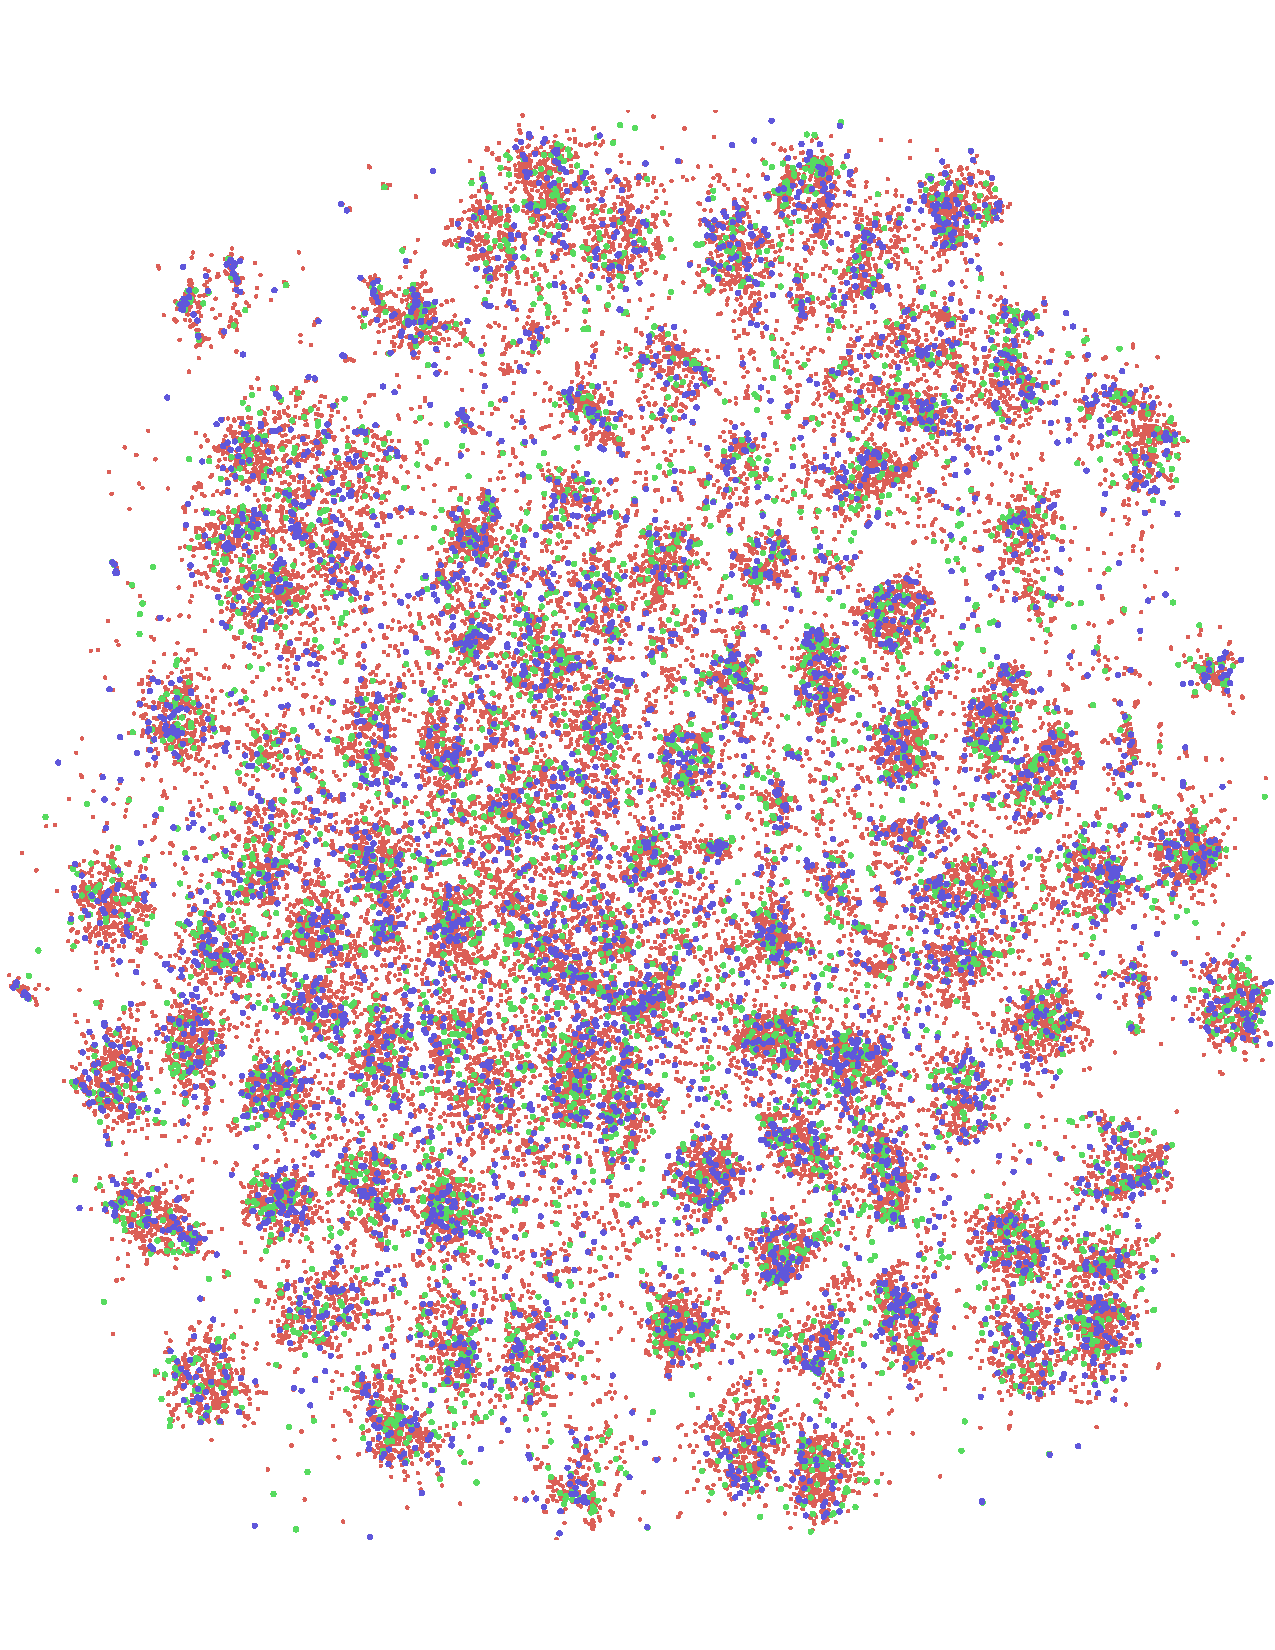
\includegraphics[width=\columnwidth]{fig1_b_1.pdf}
		\vspace{-7mm}
		\caption{Our Method}
    \end{subfigure}
\end{center}
\vspace{-3mm}
 \caption{tSNE embeddings of the CIFAR dataset and behavior of uncertainty oracle as well as our method. For both methods, the initial labeled pool of 1000 images are shown in blue, 1000 images chosen to be labeled in green and remaining ones in red. Our algorithm results in queries evenly covering the space. On the other hand, samples chosen by uncertainty oracle fails to cover the large portion of the space.}
\end{wrapfigure}


\section{Conclusion} We described an active learning algorithm for CNNs. Our empirical analysis showed that classical
uncertainty based methods have limited applicability to the CNNs. We design a simple but effective active learning
algorithm for CNNs using geometric intuitions. We further validated our algorithm using both theoretical analysis and an
empirical study. Empirical results on three datasets showed state-of-the-art performance by a large margin.


\bibliography{active_learning}
\bibliographystyle{iclr2018_conference}

\end{document}
